\documentclass[useAMS,usenatbib]{mn2e}
\usepackage{footnote,graphicx,natbib,color,multirow,amsmath,url}
\voffset=-0.5in
\pdfminorversion=5
\setlength{\parsep}{0pt}
\setlength{\partopsep}{0pt}

\def\starpy ~{\textsc{starpy}}

\font\nbf=cmssbx10 at 12.28pt %big font for headers


\begin{document}


\title[Environmental quenching: yay or nay?]{Galaxy Zoo: Quenching timescales of group galaxies}
\author[Smethurst et al. 2015]{R. ~J. ~Smethurst,$^{1}$ C. ~J. ~Lintott,$^{1}$ and the Galaxy Zoo team \footnotemark[1]
\\ $^1$ Oxford Astrophysics, Department of Physics, University of Oxford, Denys Wilkinson Building, Keble Road, Oxford, OX1 3RH, UK 
}

\maketitle

\begin{abstract}
The environment does cause quenching. But it's not the dominant mechanism. So says GZ + SDSS + GALEX + \starpy~ on group galaxies. 
\end{abstract}

\footnotetext[1]{This investigation has been made possible by the participation of over 350,000 users in the Galaxy Zoo project. Their contributions are acknowledged at \url{http://authors.galaxyzoo.org}}

\section{Introduction}\label{sec:intro}
 
 There are many mechanisms which are proposed to cause quenching; including mergers \citep{daddi10}, mass quenching \citep{kennicutt77, peng12}, morphological quenching \citep{faber12} and the environment of a galaxy.
 
 The galaxy environment as a cause of quenching was proposed due to the correlation of both morphology \citep{dressler80} and the quenched galaxy fraction \citep{?} with environmental density. 
 
 BUT does this correlation truly imply causation? Evidence from simulations \citep{?} suggests that the environment may not be the dominant quenching mechanisms for galaxies. Perhaps the correlation of increased galaxy quenched fractions with environment is due to a combination of mergers, mass and morphological quenching. In denser environments, galaxies are more likely to encounter another galaxy in a merger scenario and large viral radii give rise to long infall times during which gas reservoirs can be depleted due to star formation.
 
 To study this we need to look at how quenching timescale changes in groups and clusters of galaxies with different properties in order to isolate the cause of the density-morphology and density-SFR correlations. 
 
\section{Data and Methods}\label{sec:data}

\subsection{Data Sources}\label{sec:photo}

In this investigation we use visual classifications of galaxy morphologies from the Galaxy Zoo 2\footnote{\url{http://zoo2.galaxyzoo.org/}} (GZ2) citizen science project \citep{GZ2}, which obtains multiple independent classifications for each optical image. The full question tree for an image is shown in Figure~1 of \citeauthor{GZ2}  The GZ2 project used $304, 022$ images from the Sloan Digital Sky Survey Data Release 7 (SDSS; \citealt{york00, abazajian09}) all classified by \emph{at least} 17 independent users, with a mean number of classifications of $\sim42$.

Further to this, we required NUV photometry from the GALEX survey \citep{martin05}, within which $\sim42\%$ of the GZ2 sample was observed, giving $126, 316$ galaxies total ($0.01 < z < 0.25$). This will be referred to as the \textsc{gz2-galex} sample. The completeness of this sample ($-22 < M_u < -15$) is shown in Figure~2 of \cite{smethurst15}. 

Observed fluxes are corrected for galactic extinction \citep{Oh11} by applying the \citet*{cardelli89} law. We also adopt $k$-corrections to $z = 0.0$ and obtain absolute magnitudes from the NYU-VAGC \citep{blanton05, padova08}.


\subsection{Group Identification}\label{sec:groups}

We used the \citet{berlind06} catalogue, which uses a friends-of-friends algorithm to identify group and cluster galaxies in the SDSS. 

\subsection{Deriving quenching parameters}\label{sec:starpy}

\textsc{starpy}\footnote{Publicly available: \url{http://github.com/zooniverse/starpy}} is a \textsc{python} code which allows the user to derive the quenching star formation history (SFH) of a single galaxy through a Bayesian Markov Chain Monte Carlo method \citep{Dan}\footnote{\url{http://dan.iel.fm/emcee/}} with the input of the observed $u-r$ and $NUV-u$ colours, a redshift, and the use of the stellar population models of \cite{BC03}.  These models are implemented using solar metallicity (varying this does not substantially affect these results; \citealt{Sme2015}) and a Chabrier IMF \citep{Chab03} but does not model for intrinsic dust. The SFH is modelled as an exponential decline of the SFR described by two parameters $[t_q, \tau]$, where $t_q$ is the time at the onset of quenching $\rm{[Gyr]}$ and $\tau$ is the exponential rate at which quenching occurs $\rm{[Gyr]}$. Under the simplifying assumption that all galaxies formed at $t=0$ $\rm{ Gyr}$ with an initial burst of star formation, the SFH can be described as: 
\begin{equation}\label{sfh}
SFR =
\begin{cases}
i_{sfr}(t_q) & \text{if } t < t_q \\
i_{sfr}(t_q) \times exp{\left( \frac{-(t-t_{q})}{\tau}\right)} & \text{if } t > t_q 
\end{cases}
\end{equation}
where $i_{sfr}$ is an initial constant star formation rate dependent on $t_q$ \citep{schawinski14, smethurst15}.  A smaller $\tau$ value corresponds to a rapid quench, whereas a larger $\tau$ value corresponds to a slower quench. We note that a galaxy undergoing a slow quench is not necessarily quiescent by the time of observation. Similarly, despite a rapid quenching rate, star formation in a galaxy may still be ongoing at very low rates, rather than being fully quenched. This SFH model has previously been shown to appropriately characterise quenching galaxies \citep{Weiner06, Martin07, Noeske07,schawinski14}. We note also that star forming galaxies in this regime are fit by a constant SFR with a $t_q \simeq$ Age$(z)$, (i.e. the age of the Universe at the galaxy's observed redshift) with a very low probability.

The probabilistic fitting methods to these star formation histories for an observed galaxy are described in full detail in Section 3.2 of \cite{smethurst15}, wherein the \starpy ~~code was used to characterise the SFHs of each galaxy in the \textsc{gz2-galex} sample. We assume a flat prior on all the model parameters and the difference between the observed and predicted $u-r$ and $NUV-u$ colours are modelled as independent realisations of a double Gaussian likelihood function (Equation 2 in \citealt{smethurst15}). We also make the simplifying assumption that the age of each galaxy, $t_\mathrm{age}$ corresponds to the age of the Universe at its observed redshift, $t_\mathrm{obs}$.

The output of \starpy  ~ is probabilistic in nature and provides the posterior probability distribution across the two-parameter space for an individual galaxy the degeneracies for which can be seen in Figure~4 of \citet{smethurst15}.

\section{Results}\label{sec:results}

\begin{figure}
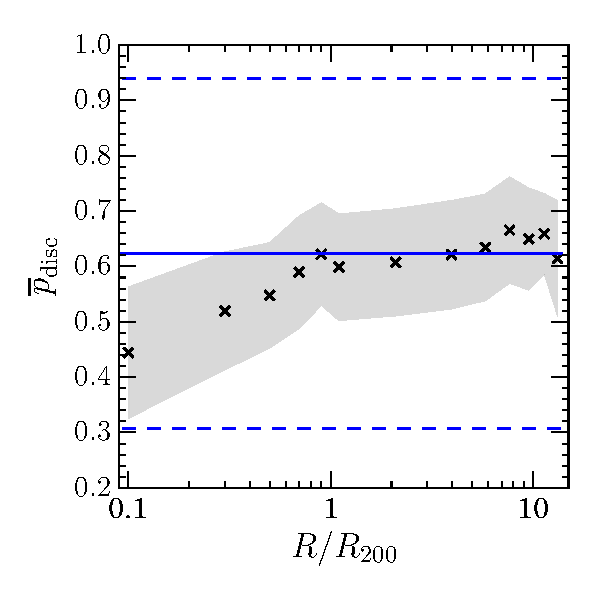
\includegraphics[width=0.46\textwidth]{p_disc_trend_with_log_radius_field_compare.pdf}
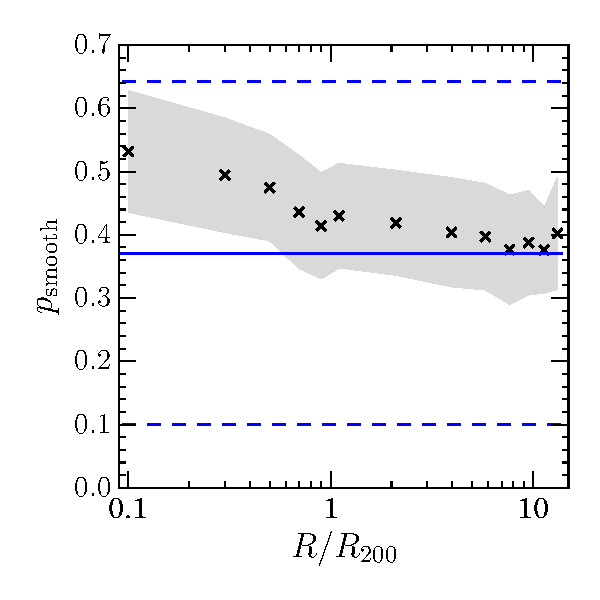
\includegraphics[width=0.46\textwidth]{p_smooth_trend_with_log_radius_field_compare.pdf}
\caption{Mean GZ vote fraction for disc (top) and smooth (bottom) galaxies in the \textsc{gz-group} sample binned in projected cluster centric radius, normalised by $R_{200}$, a proxy for the virial radius of a group.}
\label{fig:morphradius}
\end{figure}

\begin{figure}
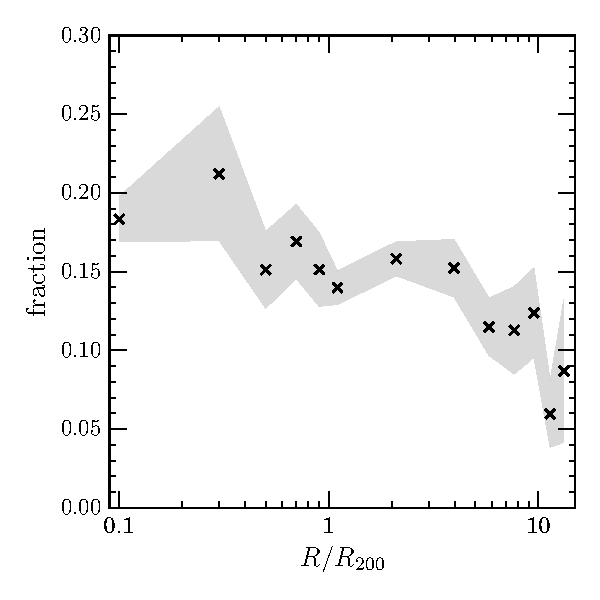
\includegraphics[width=0.46\textwidth]{bar_fraction_over_disc_trend_with_log_radius.pdf}
\caption{Bar fraction (over number of discs) in the \textsc{gz-group} sample binned in projected cluster centric radius, normalised by $R_{200}$, a proxy for the virial radius of a group.}
\label{fig:barradius}
\end{figure}

\begin{figure}
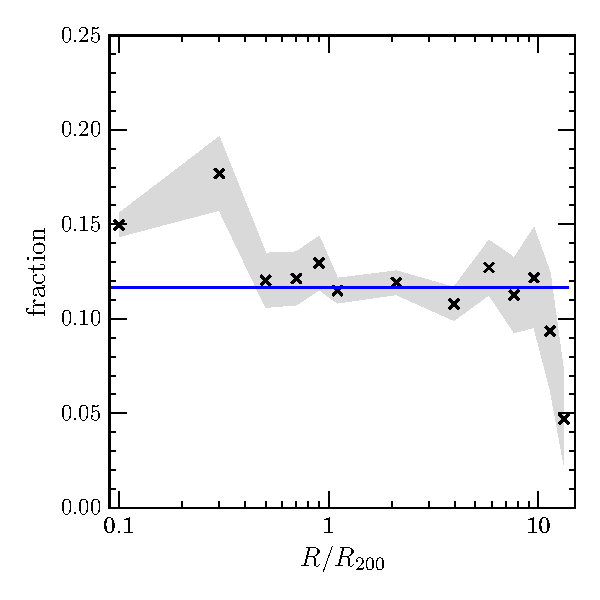
\includegraphics[width=0.46\textwidth]{merger_fraction_trend_with_log_radius_compare_field.pdf}
\caption{Merger fraction in the \textsc{gz-group} sample binned in projected cluster centric radius, normalised by $R_{200}$, a proxy for the virial radius of a group.}
\label{fig:mergerradius}
\end{figure}


\begin{figure*}
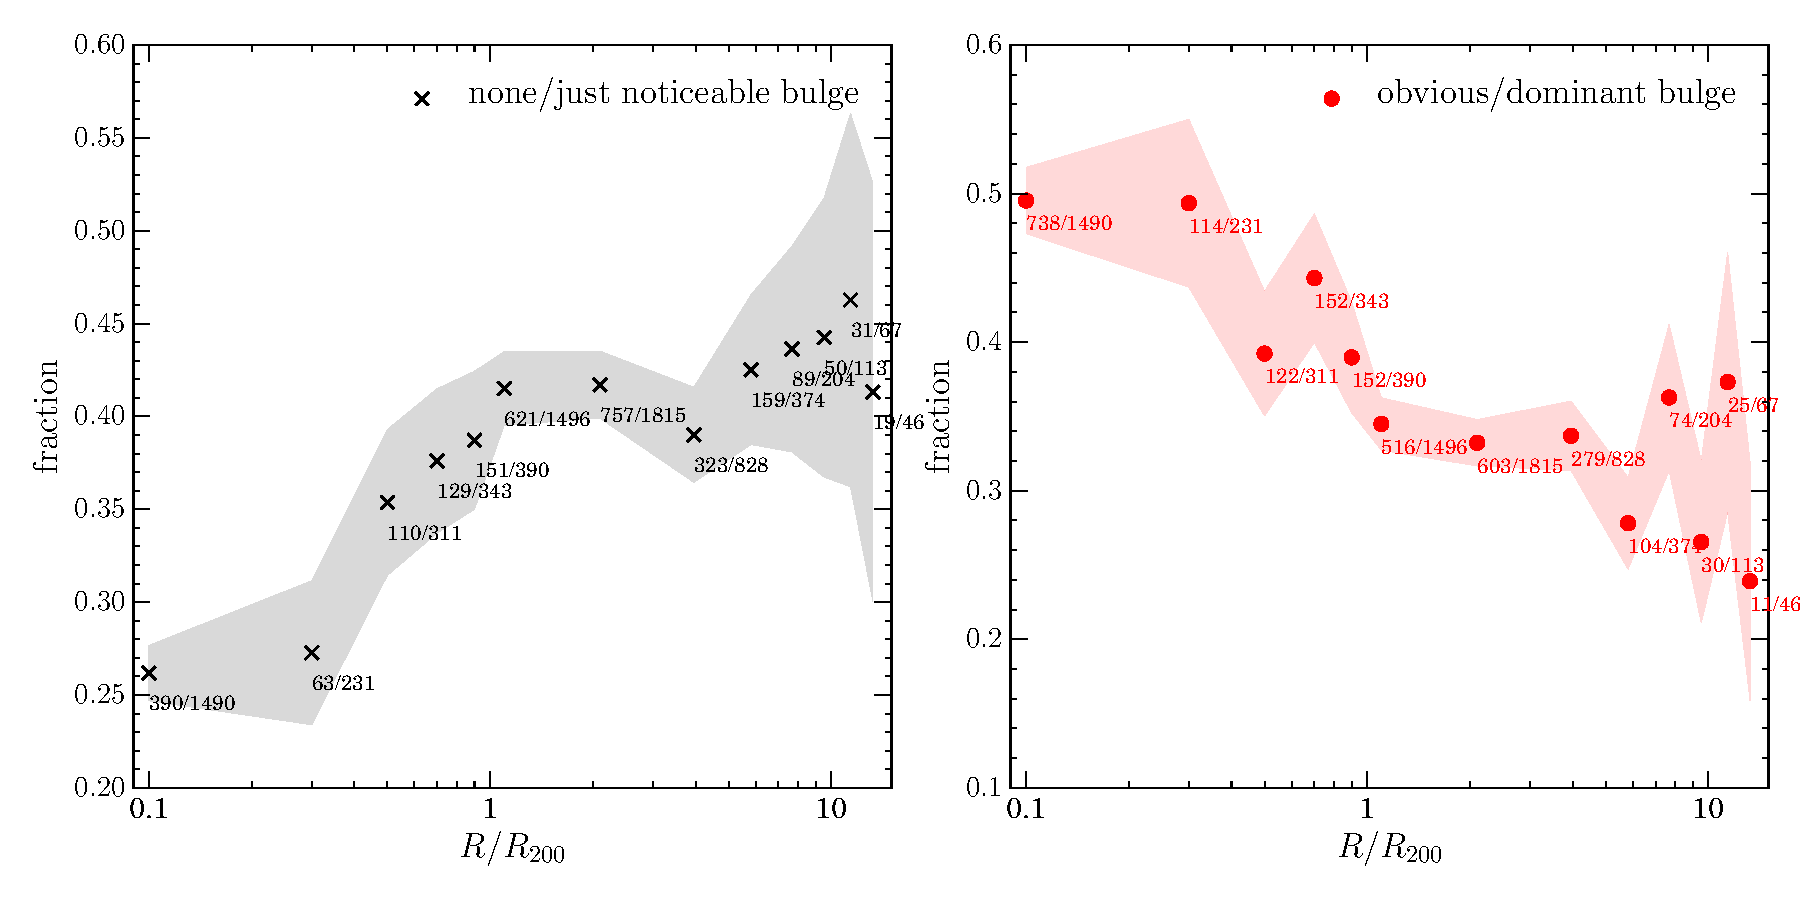
\includegraphics[width=0.8\textwidth]{min_max_bulge_fraction_trend_with_log_radius.pdf}
\caption{}
\label{fig:bulgeradius}
\end{figure*}

\begin{figure}
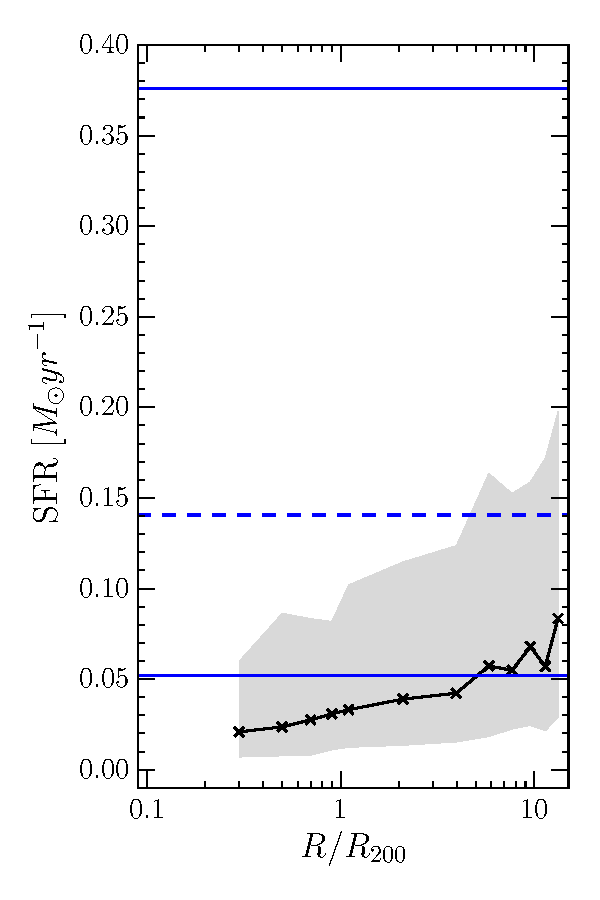
\includegraphics[width=0.46\textwidth]{sfr_trend_with_log_radius_field_matched_blue_hlines_gomez_03_rv_not_r200.pdf}
\caption{}
\label{fig:sfrradius}
\end{figure}

\begin{figure}
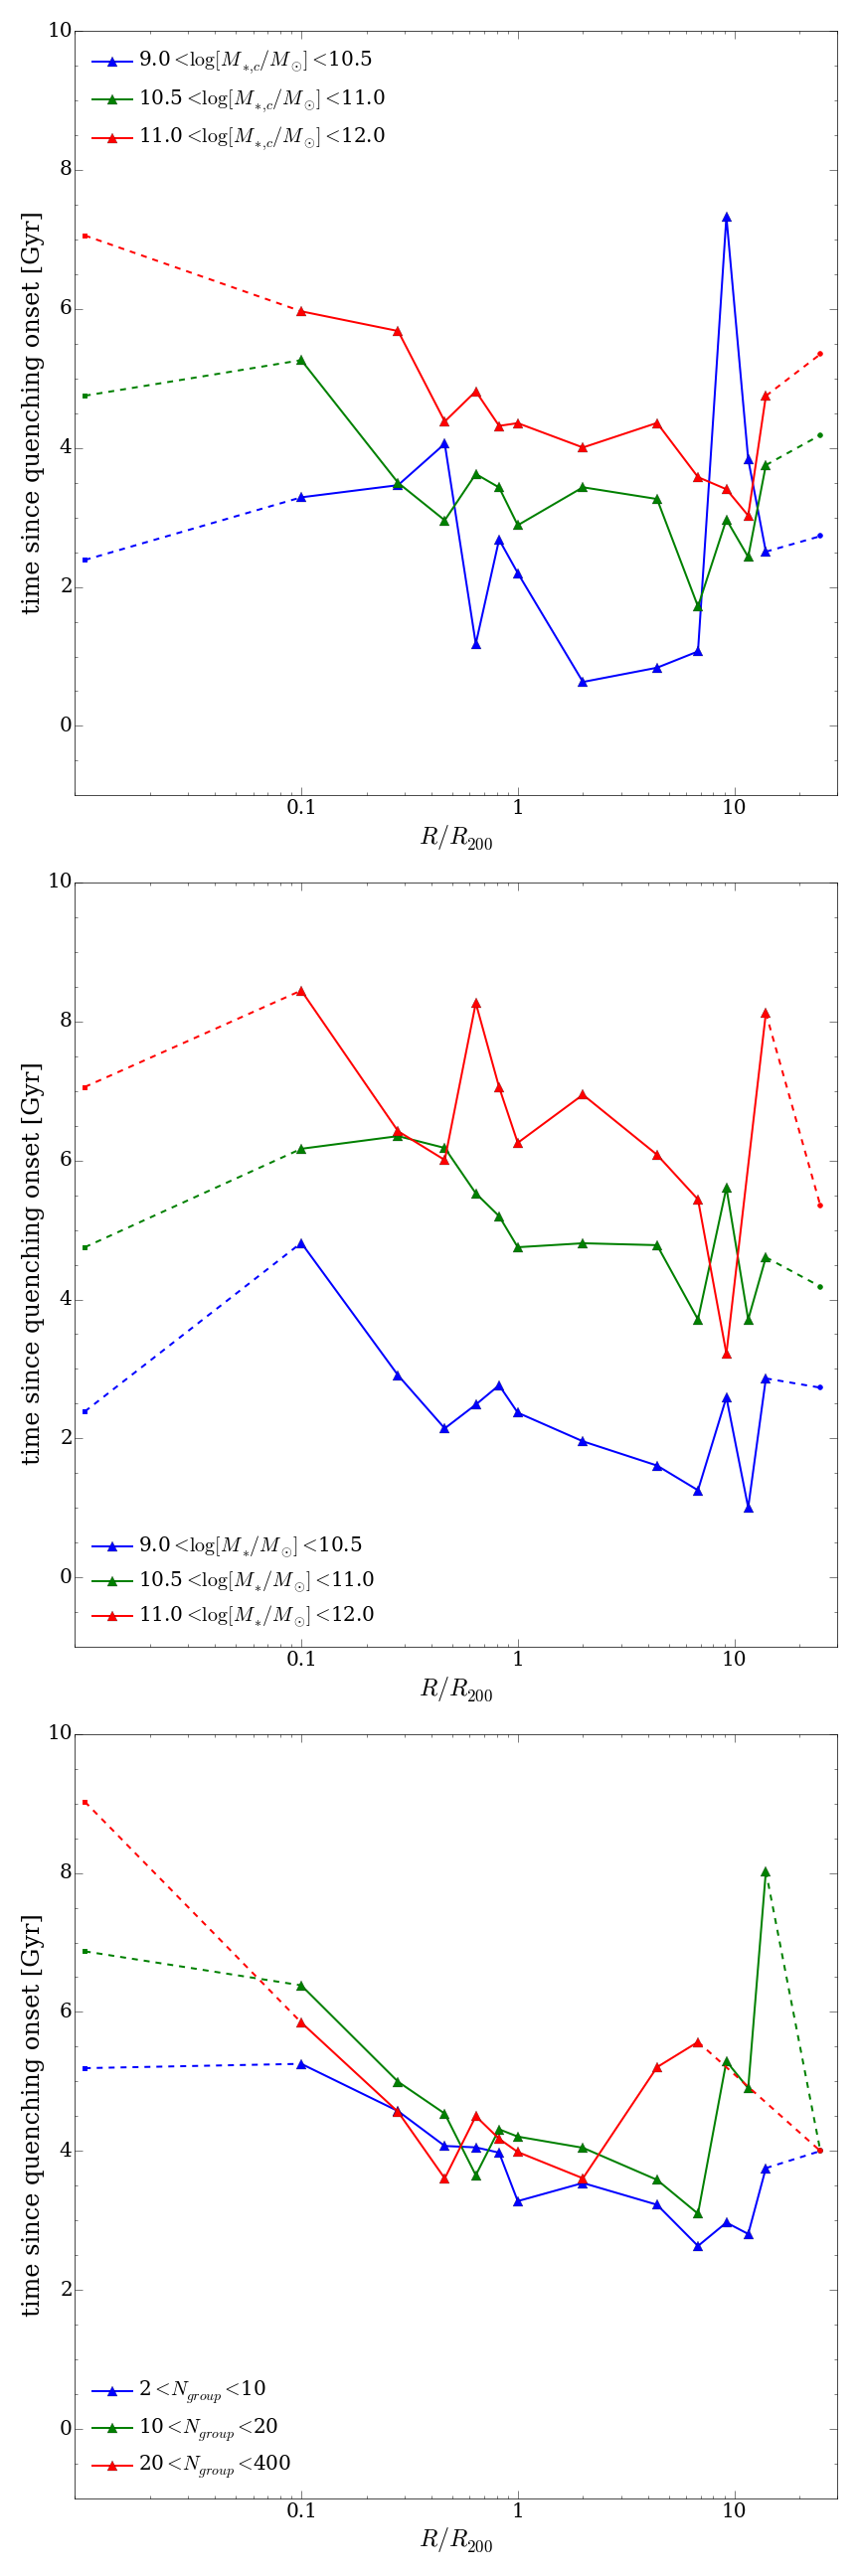
\includegraphics[height=\textheight]{time_since_quenching_environment_properties_three.png}
\caption{}
\label{fig:timesinceradius}
\end{figure}

\begin{figure}
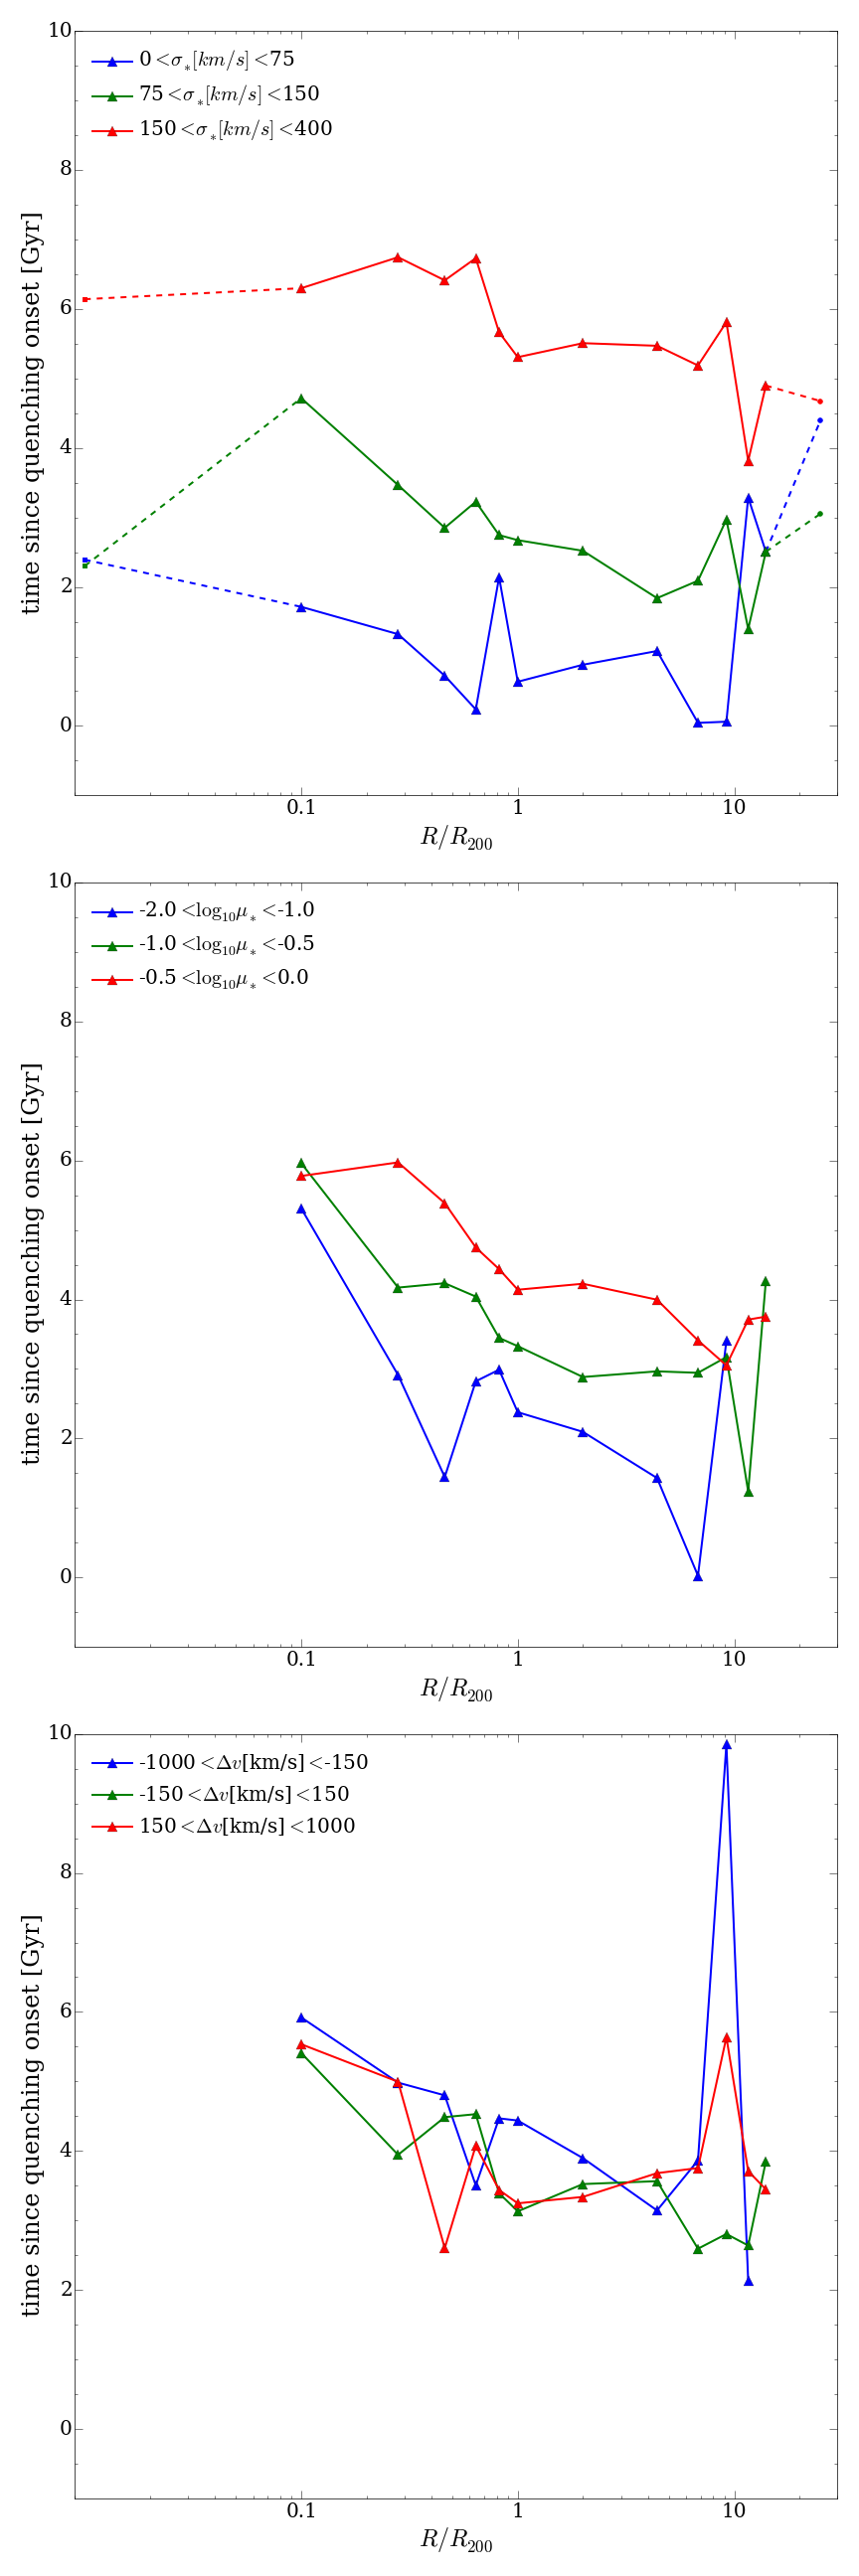
\includegraphics[height=\textheight]{time_since_quenching_v_disp_mu_bins_delv.png}
\caption{}
\label{fig:timesinceradiusvel}
\end{figure}

First start with a sanity check - do we reproduce morphology-density relation of \citet{dressler80}? Figure \ref{fig:morphradius} shows the mean disc and smooth vote fractions from galaxy zoo, binned in projected cluster centric radius (normalised by the approximate viral radius of each group, $R_{200}$). We can see that the mean disc (smooth) vote fraction decreases (increases) from the mean field value (blue line) past $1$ virial radius.

Figure \ref{fig:barradius} shows how the bar fraction (number of barred disc galaxies / number of disc galaxies) increases towards the centre of the group population suggesting the possibility that the environment may play a role in triggering the disk instabilities which produce a morphological bar \citep{ref, ref, ref}. 

Figure \ref{fig:merger radius} shows how the merger fraction does not significantly deviate from the field fraction (blue line) until beyond $1$ virial radius. Similarly in Figure \ref{fig:bulgeradius} the left panel shows how those galaxies identified as having no or just noticeable bulges are less common in the inner regions of the cluster (left panel), whereas the fraction of galaxies with obvious or dominant bulges (thought to be grown by mergers ;\citep{ref, ref, ref}) increases with decreasing projected distance from the centre of the cluster 



\section{Discussion}\label{sec:disc}

\section{Conclusions}\label{sec:conc}




\bibliographystyle{mn2e}
\bibliography{refs}  

\end{document}